% Presentation of the developed work
% Obtained Results
% Data presented in the form of figures, tables or graphs


\chapter{Results and Discussion}

In this chapter, we benchmark the selected models on NegotiationArena (Section~\ref{sec:results-benchmark}), comparing families, tiers, and roles, and relating the observed patterns to those reported by \textcite{bianchi_how_2024}. We then investigate the effect of social personas (Section~\ref{sec:results-personas}) and examine the effect of the two proposed inference-time techniques: self-refine (Section~\ref{sec:results-self-refine}) and team-based negotiation (Section~\ref{sec:results-team}).
 
\section{Open-Weight Benchmark} \label{sec:results-benchmark}



\subsection{Completion and Parse-Error Self-Correction}

% WHY DO GAMES FAIL? WHO FAILS THE MOST?

Every game depends on the model's ability to follow the protocol and output the correct XML tags. A single missing tag can cause a game to fail prematurely, which is a problem for small open-weight models. For example, without self-correction, more than a quarter of BuySell games (27.8\%) and nearly a fifth of Trading games (19.4\%) end prematurely at the very-small tier.

Surprisingly, as shown in Table~\ref{tab:cross-play-completion}, completion rate does not scale uniformly with model size. The small tier is the most reliable, with at least 96\% completion in all three games, while the medium tier falls to 67.8\% in Trading and 86.7\% in the Ultimatum Game. Failures are also unevenly distributed across models: \texttt{Gemma-3-4B-it} alone accounts for 69 parse errors, followed by \texttt{Qwen-3.5-27B} (45) and \texttt{Mistral-Small-3.2-24B} (43).

\begin{table}
\centering
\small
\caption{Parse/protocol completion rate in the benchmark cross-play experiments. Each cell pools the ordered cross-play pairings for a game and parameter tier.}
\label{tab:cross-play-completion}
\begin{tabular}{llcc}
\toprule
\textbf{Game} & \textbf{Tier} & \textbf{No retries} & \textbf{Retry-3} \\
\midrule
\multirow{3}{*}{Trading}
  & 4--9B   & 0.806 & 0.906 \\
  & 12--14B & 0.956 & 1.000 \\
  & 24--27B & 0.678 & 0.994 \\
\midrule
\multirow{3}{*}{Ultimatum}
  & 4--9B   & 0.944 & 0.994 \\
  & 12--14B & 1.000 & 1.000 \\
  & 24--27B & 0.867 & 1.000 \\
\midrule
\multirow{3}{*}{BuySell}
  & 4--9B   & 0.722 & 0.950 \\
  & 12--14B & 1.000 & 1.000 \\
  & 24--27B & 0.944 & 1.000 \\
\bottomrule
\end{tabular}
\end{table}

The main reasons for failure are game-specific. In Trading, games end mainly due to a missing \texttt{<player answer>} tag (47 games) or unparseable resource amounts (26). BuySell parse errors come mostly from a malformed trade line (40), and Ultimatum failures are usually due to a missing \texttt{<move>} tag.

% DOES OUR RETRY LOOP WORK? IF SO DOES IT CHANGE RESULTS?

The self-correction loop (Figure~\ref{fig:retry_loop}) corrects most malformed moves. Of the 9.7\% of moves that triggered a self-correction loop, 74.9\% were fixed on the first retry and 93.2\% within the three-retry budget. Only 28 games still failed to complete, mostly those involving Gemma models. Qwen triggered most of the retries (284 of 414) but almost always recovered (Figure~\ref{fig:retried-moves-resolution}).

\begin{figure}
    \centering
    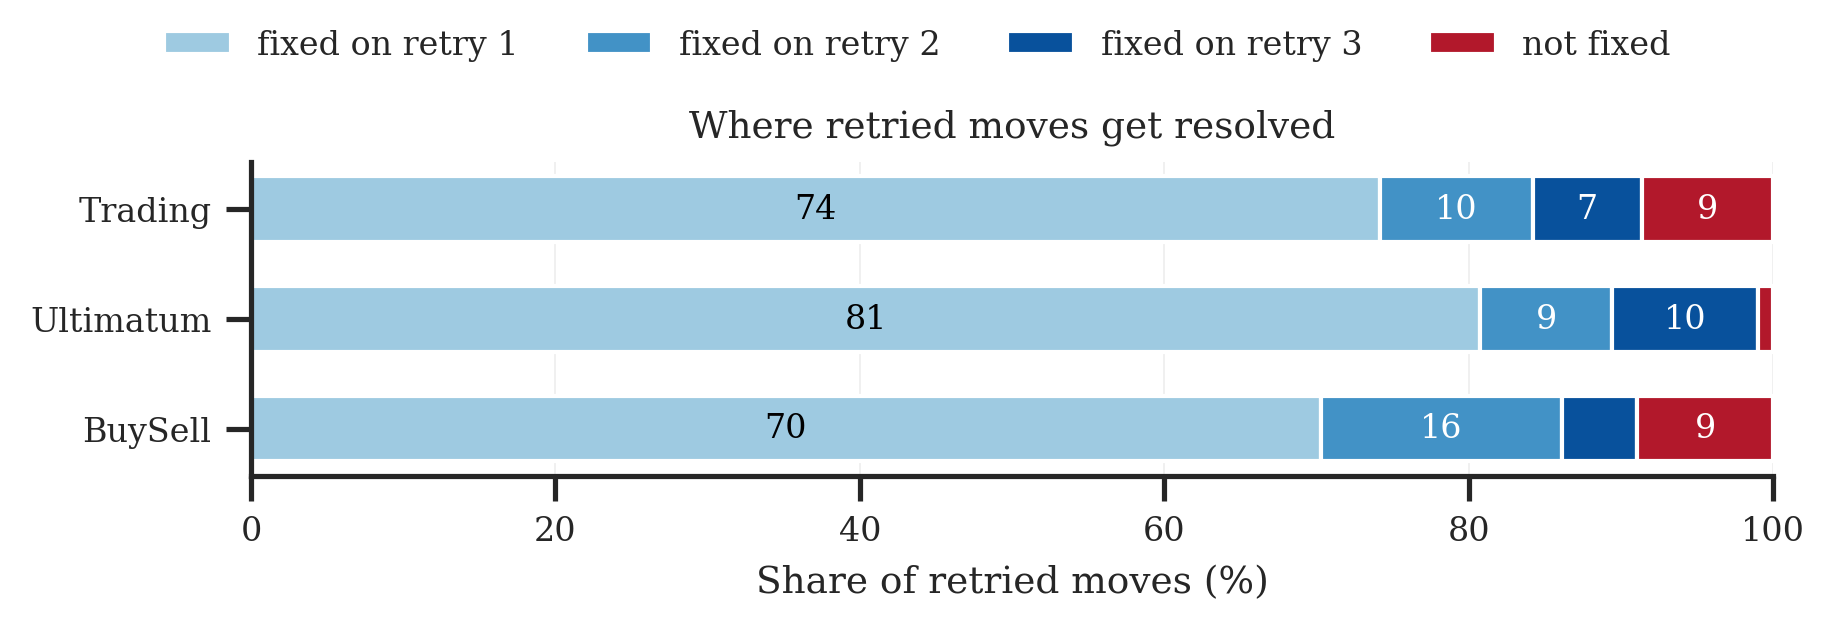
\includegraphics[width=0.8\linewidth]{figures/results/cross_play/retried_moves_resolution.png}
    \caption{Retry-3 recovery breakdown. Most corrected moves parse after one retry.}
    \label{fig:retried-moves-resolution}
\end{figure}

Self-correction does not materially change the ranking. Comparing win rates under no retries and retry-3 gives a Spearman correlation of $\rho = 0.92$ between the two conditions. Because the retry loop preserves outcomes while recovering lost games, the rest of the chapter focuses on the retry-3 results.

\subsection{Model-Family Performance}

\subsection{Role and Turn}

\subsection{Game-Specific Findings}

\paragraph{Trading.}

\paragraph{Ultimatum.}

\paragraph{BuySell.}

\section{Social Personas} \label{sec:results-personas}
\section{Self-Refine} \label{sec:results-self-refine}
\section{Team Negotiation} \label{sec:results-team}
